%!TEX root = ../main.tex

A node can be any kind of microcontroller, but this section will only address the case where a Zybo board is used as node microcontroller. 
The requirements state that it should be simple to add nodes to the system. 
To realize this the node software should be designed to be modular.
It should be easily identified what software and what interface a developer of a new node must adhere to.


\subsection{Sensor Node}\label{sec:sensor_node}
An example of a node can be seen in figure \ref{fig:gps_node}.

\mikkel{Where to put this text?}

The coming sections will explain the design of the node software that will provide the mentioned functionality using the design requirement.


\begin{figure}[!h]
\centering
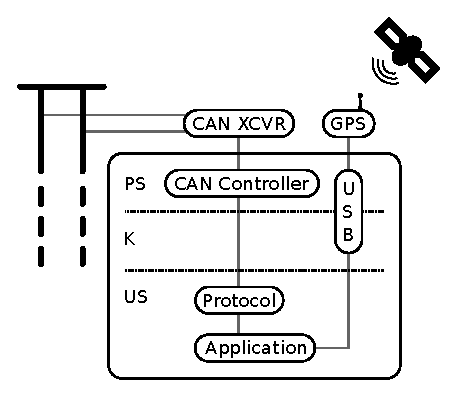
\includegraphics[width=0.5\textwidth]{graphics/analysis_gps.eps}
\caption{GPS node implemented on Zybo board.}
\label{fig:gps_node}
\end{figure}
\mikkel{Maybe change this figure to reflect the real system???}

This specific node has a GPS attached to it connected through a USB interface, but in general it could be any kind of data producing unit connected through any kind of interface.
From the analysis section is it clear that a sensor node has the following responsibilities:

\begin{itemize}
\item Get data from associated sensor.
\item Pack data according to the specified protocol.
\item Construct CAN package
\item Send data using a CAN controller.
\item Get data from CAN network.
\item React to commands sent to it.
\end{itemize}
As described earlier the responsibility of sending data using a CAN controller and receiving data from the CAN network is done in the earlier in the described bare-metal code.
This section will focus on the designing and implementing the code that implements the rest of the listed functionality.

Analyzing on the procedure when data goes from a sensor to the CAN program resulted in the block diagram of figure \ref{fig:block_gps}.

\begin{figure}[!h]
\centering
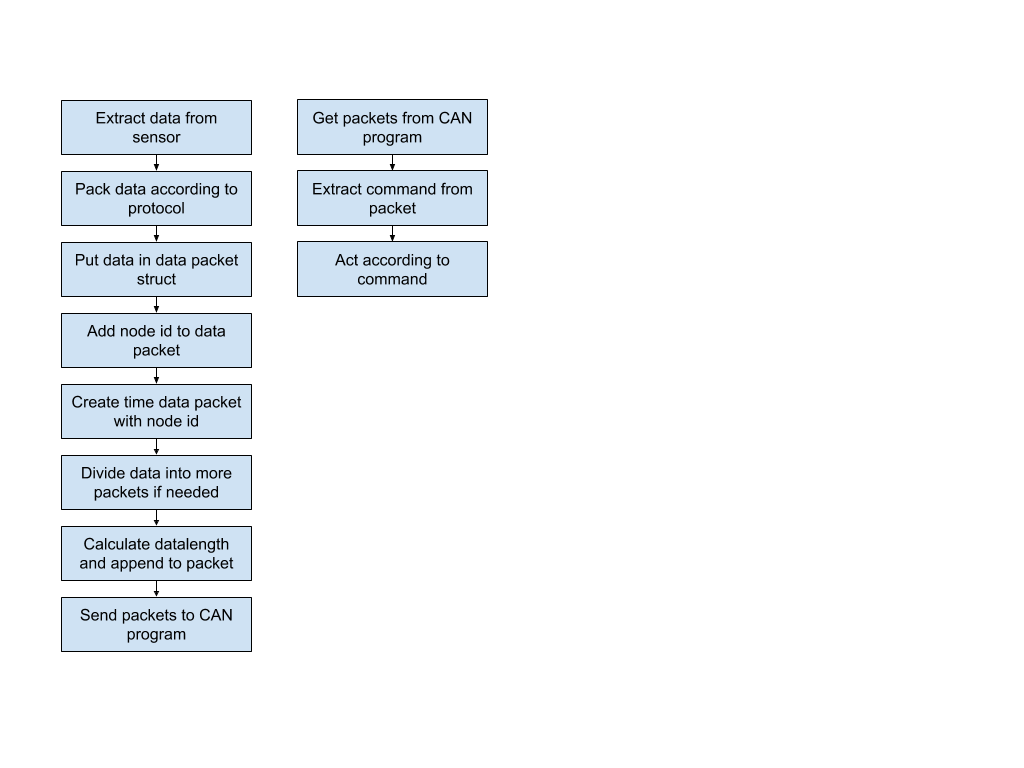
\includegraphics[width=1\textwidth]{graphics/block_diagram.png}
\caption{.....}
\label{fig:block_gps}
\end{figure}

To design modular software it needs to be analyzed which blocks are the same for all nodes and which are sensor specific.
The sensor specific tasks are found to be extracting data from sensor and to pack data according to the protocol.
The remaining tasks are the same for all sensor nodes in the system. 
The procedure when data is going from the CAN program to the node is shown in figure \ref{fig:block_gps}.
All tasks are found to be generic for all sensor nodes.

\subsubsection*{Class diagram}
Based on the previous analysis a class diagram was developed and can be seen in figure \ref{fig:node_class_diagram}.
Classes to the right of the dashed horizontal is sensor specific and should be developed for each specific sensor.
Classes to the left are agnostic to all data they receive going from the sensor and to the CAN network.
They are generic classes and should be reused when developing new nodes.

\begin{figure}[!h]
\centering
\missingfigure[figwidth=1\textwidth]{Class diagram}
\caption{Class diagram showing node software.}
\label{fig:node_class_diagram}
\end{figure}

A struct containing all fields of a data packet in boolean data types is defined in listing \ref{code:data_packet}.  

\begin{lstlisting}[caption=Struct for data packet.,label=code:data_packet]
struct data_packet {
  std::bitset<1> sof;
  std::bitset<4> node_id;
  std::bitset<4> n_data_bytes;
  std::bitset<6> messagetype;
  std::vector<bool> data;
(*@\makebox[\linewidth][c]{$\smash{\vdots}$}@*)
};
\end{lstlisting}
It will be passed between the classes and they will each add their own information. 

The classes and their tasks from figure \ref{code:data_packet} will be explained here.

~\\ \par \textbf{GPS class} ~ \\
The GPS class needs to extract data from a connected GPS unit and update its own variables with that data.
The specific GPS unit used in this project has a USB interface and uses the NMEA protocol to format data.

~\\ \par \textbf{Packer\_GPS class} ~ \\
The Packer\_GPS class is also sensor specific and is the link between the sensor and the data agnostic node.
It is hard-coded with the message types that the sensor is allowed to send onto the network.
It has the responsibility to pack data according to the developed protocol.
The reason for making a separate class for the packer and not putting the functionality into the GPS class is that if the specification of the protocol or message types change, only this class needs to be modified.

~\\ \par \textbf{Node class} ~ \\
The Node class receives data in a vector of booleans from the Packer class.
The class needs to put the received data in a data\_packet struct and append its node id to it.
It needs to create a timestamp data\_packet each time data is to be sent.
In order to create the time message the class needs to keep track of milliseconds since last received synchronize message.
The class receives start, stop or synchronize events from the protocol class and reacts to those accordingly.

~\\ \par \textbf{Protocol class} ~ \\
The protocol class receives data\_packets from the node class. 
If it receives data\_packets where there are more than eight data bytes it needs to create additional data\_packets and distribute data to them. 
The additional data\_packets must have the same node id and message types, but the start of frame, sof, bit should be set accordingly.
The class also needs to append number of data bytes, n\_data\_bytes, to each data\_packet.
On data\_packets coming from the CAN network the class needs to use the last two bits of the messagetype to decode which command is sent to the node.
\martin{This may or may not be adressed to the node, so it should be handled in node.}

~\\ \par \textbf{CAN\_link class} ~ \\
The CAN\_link class has the responsibility of transferring and receiving data to and from the CAN program.
As this interface has not yet been implemented this class makes use of the standard input and output. 
Meaning that data from the sensor will be printed in the shell and data to the node should be written to the shell. 

\subsubsection*{Passing data between classes}
Threads, buffer and mutexes.
Communication between classes is realised by having buffers for all data going into a class.
The buffers will be read by looping functions running in separate threads.
All buffers have a associated mutex to the implementation thread safe.

\subsection{Wifi Node}
\mikkel{We should design something or at least make some block diagrams of what needs to happen with data here.}


\catalin{Explain the code in more detail}
\mikkel{This should not be here}
\subsection{CAN Controller Software}
\subsubsection{Implementation in code}~\\
As mentioned in section \ref{sub:Basic_SourceCode}, the code was based on the xcanps polled example available by Xilinx documentation.
The important functionalities that needed to be provided by the final software version included:

\begin{itemize}
\item receiving and sending of frames
\item the creation of the message id
\item the decoding of the message id parts, such as the node id, the message type etc. \catalin{what else?}
\item handling button interrupts
\item controlling the LEDs
\item subscriptions lookup
\end{itemize}
\catalin{What other functionalities? And, 1st letters capitals or not?}
The figure \ref{fig:SeqDiagram_SendFrame} shows the procedure of sending a frame to the CAN network containing data, which makes use of the protocol function createMsgID().
After returning the message id, the id and the data are put into the TxFrame to be sent once the FIFO has space.
The actual sending is done with a call to the XCanPs function XCanPs\_Send().
\\
Similarly, the procedure of receiving a frame is shown in the figure \ref{fig:SeqDiagram_RecvFrame}.
The node once it calls the RecvFrame() function, it waits in a loop until it receives a frame. Then, it checks the subscriptions in order to forward the packet for further processing or to ignore it.


This was achieved by implementing a set of functions and an array variable of subscriptions for each node.

\begin{figure}[h!]
	\centering
	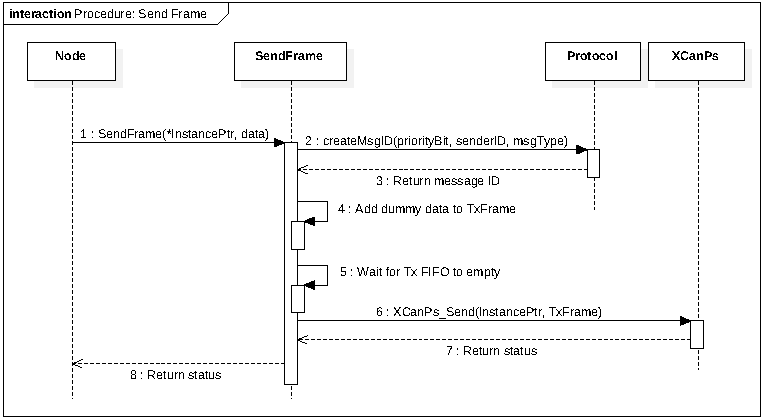
\includegraphics[width = 1.1\linewidth]{graphics/SeqDiagram_SendFrame.pdf}
	\caption{The sequence diagram of the process of sending a frame.}
	\label{fig:SeqDiagram_SendFrame}
\end{figure}

\begin{figure}[h!]
	\centering
	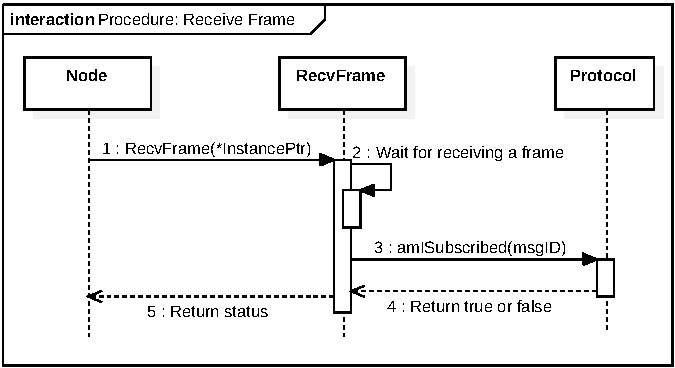
\includegraphics[width = 1.1\linewidth]{graphics/SeqDiagram_RecvFrame.pdf}
	\caption{The sequence diagram of the process of receiving a frame.}
	\label{fig:SeqDiagram_RecvFrame}
\end{figure}



\begin{figure}[h!]
	\centering
	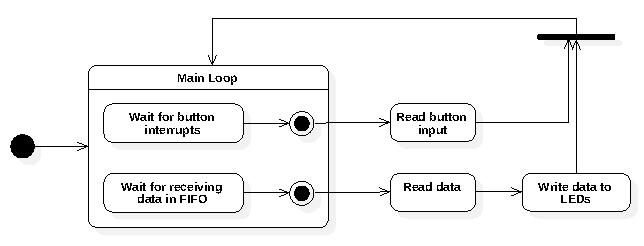
\includegraphics[width = 1.1\linewidth]{graphics/StateDiagram_CanStackTestCode.pdf}
	\caption{Behavioral diagram of the basic source code.}
	\label{fig:CAN_Testing_StateDiagr_Code}
\end{figure}